\documentclass{beamer}
\usetheme{Singapore}
\usepackage{amsmath}
\usepackage{hyperref}
\usepackage{breakurl}

\setbeamertemplate{footline}[frame number]

\begin{document}
	\title{A $\rightarrow$ Z h Analysis Tutorial}
	\subtitle{Level 1 and Level 2}
	\author{Nikola Whallon}
	\institute{University of Washington}
	\date{6/25/14}
%%%%%%%%%%%%%%%%%%%%%%%%%%%%%%%%%%%%%%%%%%%%%%%%%%%%%%%%%%%%%%%%%%%%%%%%%%%%%%%%%%%%%%%%%%%%%%%%%%%%%%%%%%%%%%%%%%%%%%%%%%%%%%%%%%%%%%%%%%%%%%%%%%%%%%%%%%%%%%%%%%%%%%%%%%%%%%%%%%%%%%%%%%%%%%%%%%%
	\frame{\titlepage}
%%%%%%%%%%%%%%%%%%%%%%%%%%%%%%%%%%%%%%%%%%%%%%%%%%%%%%%%%%%%%%%%%%%%%%%%%%%%%%%%%%%%%%%%%%%%%%%%%%%%%%%%%%%%%%%%%%%%%%%%%%%%%%%%%%%%%%%%%%%%%%%%%%%%%%%%%%%%%%%%%%%%%%%%%%%%%%%%%%%%%%%%%%%%%%%%%%%
	\begin{frame}{A $\rightarrow$ Z h Tutorial Motivation and Purpose}
		\begin{itemize}
\item<1->The A $\rightarrow$ Z h (AZH) Analysis Tutorial is built as a ground up tutorial to teach users the basics of Montecarlo simulation and data analysis of particle physics processes.

\bigskip

\item<1->While the tutorial studies the hypothetical AZH process with the 2HDM4TC model, the techniques presented in the tutorial are applicable to any particle physics process.

\bigskip

\item<1->Performing simulations of hypothetical particle physics models is critical in understanding the predictions of those models, allowing the models to be tested in experiments such as ATLAS.
		\end{itemize}
	\end{frame}
%%%%%%%%%%%%%%%%%%%%%%%%%%%%%%%%%%%%%%%%%%%%%%%%%%%%%%%%%%%%%%%%%%%%%%%%%%%%%%%%%%%%%%%%%%%%%%%%%%%%%%%%%%%%%%%%%%%%%%%%%%%%%%%%%%%%%%%%%%%%%%%%%%%%%%%%%%%%%%%%%%%%%%%%%%%%%%%%%%%%%%%%%%%%%%%%%%%
	\begin{frame}{A $\rightarrow$ Z h Analysis Tutorial Contents}
		\begin{itemize}
\item<1->The tutorial consists of a main AZH Tutorial pdf, presentations (like this one), and a code base documented with comments and README files. All of this is maintained in the following git repositories.

\bigskip

\url{https://github.com/schsu/PhysAna-AtoZh}

\url{https://github.com/schsu/DelphesJetSubstructure}

\bigskip

\item<1->An outline of the tutorial can be found on the following sharepoint page.

\bigskip

\url{https://sharepoint.washington.edu/phys/wiki/tev-cluster/Pages/Analysis/Analysis101.aspx}

\bigskip

\item<1->Some of these resources are still incomplete, but it is my goal to work on making the tutorial thorough and complete this summer.
		\end{itemize}
	\end{frame}
%%%%%%%%%%%%%%%%%%%%%%%%%%%%%%%%%%%%%%%%%%%%%%%%%%%%%%%%%%%%%%%%%%%%%%%%%%%%%%%%%%%%%%%%%%%%%%%%%%%%%%%%%%%%%%%%%%%%%%%%%%%%%%%%%%%%%%%%%%%%%%%%%%%%%%%%%%%%%%%%%%%%%%%%%%%%%%%%%%%%%%%%%%%%%%%%%%%
	\begin{frame}{A $\rightarrow$ Z h Analysis Tutorial Outline}
The tutorial is broken up into the following 4 sections.

\bigskip

		\begin{itemize}
\item<1-> Level 1: Generating Simulated Events with 2HDM4TC
\item<1-> Level 2: Truth Particle Study
\item<1-> Level 3: Detected Particle Study
\item<1-> Level 4: Jet Substructure Study
		\end{itemize}

\bigskip

In this presentation I will discuss Level 1 and Level 2 and present some of my results on an inclusive study of truth particle data of simulated AZH events.
	\end{frame}
%%%%%%%%%%%%%%%%%%%%%%%%%%%%%%%%%%%%%%%%%%%%%%%%%%%%%%%%%%%%%%%%%%%%%%%%%%%%%%%%%%%%%%%%%%%%%%%%%%%%%%%%%%%%%%%%%%%%%%%%%%%%%%%%%%%%%%%%%%%%%%%%%%%%%%%%%%%%%%%%%%%%%%%%%%%%%%%%%%%%%%%%%%%%%%%%%%%
	\begin{frame}{Level 1: Generating Simulated Events with MadGraph, Pythia, Delphes, and 2HDM4TC}
		\begin{itemize}
\item<1->MadGraph, Pythia, and Delphes are software packages which perform Montecarlo simulations of particle physics processes. The purpose of Level 1 in the AZH Tutorial is to guide the user through proper installation and configuration of these packages and the 2HDM4TC Model in order to generate a Montecarlo simulation of our AZH process.

\bigskip

\item<1->The technical details of setting up these packages are given in the AZH Tutorial pdf. Here I will describe the role of each package in the Montecarlo simulation process. I will also discuss the use of the configuration files used by these packages to tune your simulation.
		\end{itemize}
	\end{frame}
%%%%%%%%%%%%%%%%%%%%%%%%%%%%%%%%%%%%%%%%%%%%%%%%%%%%%%%%%%%%%%%%%%%%%%%%%%%%%%%%%%%%%%%%%%%%%%%%%%%%%%%%%%%%%%%%%%%%%%%%%%%%%%%%%%%%%%%%%%%%%%%%%%%%%%%%%%%%%%%%%%%%%%%%%%%%%%%%%%%%%%%%%%%%%%%%%%%
	\begin{frame}{MadGraph}
		\begin{itemize}
\item<1->MadGraph simulates particle physics processes, such as the process we are interested in:

\bigskip

$p p \rightarrow{} A$, $A \rightarrow{} Z h$, $h \rightarrow{} b \bar{b}$, $Z \rightarrow{} l+ l-$

\bigskip

\item<1->MadGraph takes a file defining the physical process as input, and outputs a Les Houches Event (LHE) file containing simulated events as output. The output is all parton level - meaning, for example, in our process here, $b$ and $\bar{b}$, rather than jets, show up as particles in the output.
		\end{itemize}
	\end{frame}
%%%%%%%%%%%%%%%%%%%%%%%%%%%%%%%%%%%%%%%%%%%%%%%%%%%%%%%%%%%%%%%%%%%%%%%%%%%%%%%%%%%%%%%%%%%%%%%%%%%%%%%%%%%%%%%%%%%%%%%%%%%%%%%%%%%%%%%%%%%%%%%%%%%%%%%%%%%%%%%%%%%%%%%%%%%%%%%%%%%%%%%%%%%%%%%%%%%
	\begin{frame}{Partons and Parton Showers}
		\begin{itemize}
\item<1->A parton is a model for the constituents of hadrons such as protons. The parton model has been used longer than the validation of the quark model, and since, partons have been matched to quarks and gluons.

\bigskip

\item<1->Since quarks are not observed in isolation, the simulation process cannot end here. In nature, these color-carrying quarks and gluons accelerate, radiating gluons which in turn accelerate and radiate more gluons. This process is known as a "parton shower," and this process must be simulated next.
		\end{itemize}
	\end{frame}
%%%%%%%%%%%%%%%%%%%%%%%%%%%%%%%%%%%%%%%%%%%%%%%%%%%%%%%%%%%%%%%%%%%%%%%%%%%%%%%%%%%%%%%%%%%%%%%%%%%%%%%%%%%%%%%%%%%%%%%%%%%%%%%%%%%%%%%%%%%%%%%%%%%%%%%%%%%%%%%%%%%%%%%%%%%%%%%%%%%%%%%%%%%%%%%%%%%
	\begin{frame}{Pythia}
Pythia is the software package which simulates these parton showers. It takes an LHE file as input and outputs an LHE file and a HEP file as output. These files contain all final state particle information before the detector response is simulated.
	\end{frame}
%%%%%%%%%%%%%%%%%%%%%%%%%%%%%%%%%%%%%%%%%%%%%%%%%%%%%%%%%%%%%%%%%%%%%%%%%%%%%%%%%%%%%%%%%%%%%%%%%%%%%%%%%%%%%%%%%%%%%%%%%%%%%%%%%%%%%%%%%%%%%%%%%%%%%%%%%%%%%%%%%%%%%%%%%%%%%%%%%%%%%%%%%%%%%%%%%%%
	\begin{frame}{Delphes}
		\begin{itemize}
\item<1->Delphes is the software package which simulates the detector reponse to the final state particles of our simulated process.

\bigskip

\item<1->It is a crude simulation which applies simple reconstruction efficiencies to particles as a function of their PT and Eta, momentum and energy smearing, jet reconstruction, and jet b-tagging.

\bigskip

\item<1->The behavior of Delphes is highly configurable, and its configuration file must be fully understood in order to understand the final data output by the whole simulation process.
		\end{itemize}
	\end{frame}
%%%%%%%%%%%%%%%%%%%%%%%%%%%%%%%%%%%%%%%%%%%%%%%%%%%%%%%%%%%%%%%%%%%%%%%%%%%%%%%%%%%%%%%%%%%%%%%%%%%%%%%%%%%%%%%%%%%%%%%%%%%%%%%%%%%%%%%%%%%%%%%%%%%%%%%%%%%%%%%%%%%%%%%%%%%%%%%%%%%%%%%%%%%%%%%%%%%
	\begin{frame}{Configuration Files}
		\begin{itemize}
\item<1->MadGraph's, Pythia's, and Delphes' configuration files are called "cards," and editing these cards gives you control and understanding of your simulation process.

\bigskip

\item<1->In particular, MadGraph's parameter and run cards and Delphes' delphes card can be modified to tune our AZH study.

\bigskip

\item<1->Where to grab the right cards for AZH analysis and how to edit these cards is described in detail in the AZH Tutorial pdf. Here, I present the basic roles of the paramater, run, and delphes cards.
		\end{itemize}
	\end{frame}
%%%%%%%%%%%%%%%%%%%%%%%%%%%%%%%%%%%%%%%%%%%%%%%%%%%%%%%%%%%%%%%%%%%%%%%%%%%%%%%%%%%%%%%%%%%%%%%%%%%%%%%%%%%%%%%%%%%%%%%%%%%%%%%%%%%%%%%%%%%%%%%%%%%%%%%%%%%%%%%%%%%%%%%%%%%%%%%%%%%%%%%%%%%%%%%%%%%s
	\begin{frame}{Parameter Card}
		\begin{itemize}
\item<1->The parameter card, called param\_card.dat, contains physics parameter definitions, such as the mass of particles.

\bigskip

\item<1->Since we are probing new physics with the AZH model, our model comes with its own parameter card defining such things as the mass of A.

\bigskip

\item<1->Since the mass of A is not known, it is important to carry out our simulation studies at various masses of A. To do this, the definition of the mass of A must be modified in this parameter card before simulation.

\bigskip

\item<1->The analysis results presented in following slides come from my AZH simulation with a mass of A of 1000 GeV.
		\end{itemize}
	\end{frame}
%%%%%%%%%%%%%%%%%%%%%%%%%%%%%%%%%%%%%%%%%%%%%%%%%%%%%%%%%%%%%%%%%%%%%%%%%%%%%%%%%%%%%%%%%%%%%%%%%%%%%%%%%%%%%%%%%%%%%%%%%%%%%%%%%%%%%%%%%%%%%%%%%%%%%%%%%%%%%%%%%%%%%%%%%%%%%%%%%%%%%%%%%%%%%%%%%%%
	\begin{frame}{Run Card}
		\begin{itemize}
\item<1->The run card, called run\_card.dat, contains information about the simulated run, such has how many Events to simulate and what the energy of our p p beam is.

\bigskip

\item<1->In order to have high statistics in our analysis later on, we should simulate as many Events as possible. For technical reasons, the largest number of Events one should simulate in a run using these packages is 50000. 
		\end{itemize}
	\end{frame}
%%%%%%%%%%%%%%%%%%%%%%%%%%%%%%%%%%%%%%%%%%%%%%%%%%%%%%%%%%%%%%%%%%%%%%%%%%%%%%%%%%%%%%%%%%%%%%%%%%%%%%%%%%%%%%%%%%%%%%%%%%%%%%%%%%%%%%%%%%%%%%%%%%%%%%%%%%%%%%%%%%%%%%%%%%%%%%%%%%%%%%%%%%%%%%%%%%%
	\begin{frame}{Delphes Card}
		\begin{itemize}
\item<1->The delphes card, called delphes\_card.dat, contains parameters for detection, reconstruction, and jet b-tagging efficiencies of particles. It also contains parameters for energy and momentum smearing.

\bigskip

\item<1->In order to understand the data output by Delphes, it is important to cross check your particle efficiencies with the efficiencies defined in the delphes card. This is especially important when doing Event efficiency studies.

\bigskip

\item<1->The delphes card also contains a series of modules to execute, running the various reconstruction algorithms. Editing these modules is an advanced topic, but you should look through your delphes card to learn what each module does.
		\end{itemize}
	\end{frame}
%%%%%%%%%%%%%%%%%%%%%%%%%%%%%%%%%%%%%%%%%%%%%%%%%%%%%%%%%%%%%%%%%%%%%%%%%%%%%%%%%%%%%%%%%%%%%%%%%%%%%%%%%%%%%%%%%%%%%%%%%%%%%%%%%%%%%%%%%%%%%%%%%%%%%%%%%%%%%%%%%%%%%%%%%%%%%%%%%%%%%%%%%%%%%%%%%%%
	\begin{frame}{Generating Events}
With this overview of the software and configuration required to generate Montecarlo simulations of particle physics processes, you should be ready to read the AZH Tutorial pdf to become familiar with the technical details of generating Events to later analyze.

\bigskip

The next step in our analysis is to study the truth particle information in your generated data. This is done in Level 2 of the tutorial.
	\end{frame}
%%%%%%%%%%%%%%%%%%%%%%%%%%%%%%%%%%%%%%%%%%%%%%%%%%%%%%%%%%%%%%%%%%%%%%%%%%%%%%%%%%%%%%%%%%%%%%%%%%%%%%%%%%%%%%%%%%%%%%%%%%%%%%%%%%%%%%%%%%%%%%%%%%%%%%%%%%%%%%%%%%%%%%%%%%%%%%%%%%%%%%%%%%%%%%%%%%%
	\begin{frame}{Level 2: Truth Particle Study}
		\begin{itemize}
\item<1->With data generated in Level 1, all particles in physical process are kept track of. In the last step with Delphes, final state particles are subjected to the detector response, and may not be detected. All particles before this step are known as "truth particles."

\bigskip

\item<1->Studying the structure of an Event at the truth particle level as well as truth particle kinematics is critical in understanding the physical process before applying our detector response.

\bigskip

\item<1->Level 2 consists of 2 programs to do this: truth\_table and truth\_histogram. The AZH Tutorial pdf goes over the technical programming details of these programs. Here I will explain some of the results.
		\end{itemize}
	\end{frame}
%%%%%%%%%%%%%%%%%%%%%%%%%%%%%%%%%%%%%%%%%%%%%%%%%%%%%%%%%%%%%%%%%%%%%%%%%%%%%%%%%%%%%%%%%%%%%%%%%%%%%%%%%%%%%%%%%%%%%%%%%%%%%%%%%%%%%%%%%%%%%%%%%%%%%%%%%%%%%%%%%%%%%%%%%%%%%%%%%%%%%%%%%%%%%%%%%%%
	\begin{frame}{truth\_table}
The code for truth\_table can be found in the tutorial github repository at the following url.

\bigskip

\url{https://github.com/schsu/PhysAna-AtoZh/tree/master/level2/truth_table}

\bigskip

This program outputs a table of information on truth particles. An example output is on the following slide.
	\end{frame}
%%%%%%%%%%%%%%%%%%%%%%%%%%%%%%%%%%%%%%%%%%%%%%%%%%%%%%%%%%%%%%%%%%%%%%%%%%%%%%%%%%%%%%%%%%%%%%%%%%%%%%%%%%%%%%%%%%%%%%%%%%%%%%%%%%%%%%%%%%%%%%%%%%%%%%%%%%%%%%%%%%%%%%%%%%%%%%%%%%%%%%%%%%%%%%%%%%%
	\begin{frame}{truth\_table Output}
		\begin{figure}
			\centering
			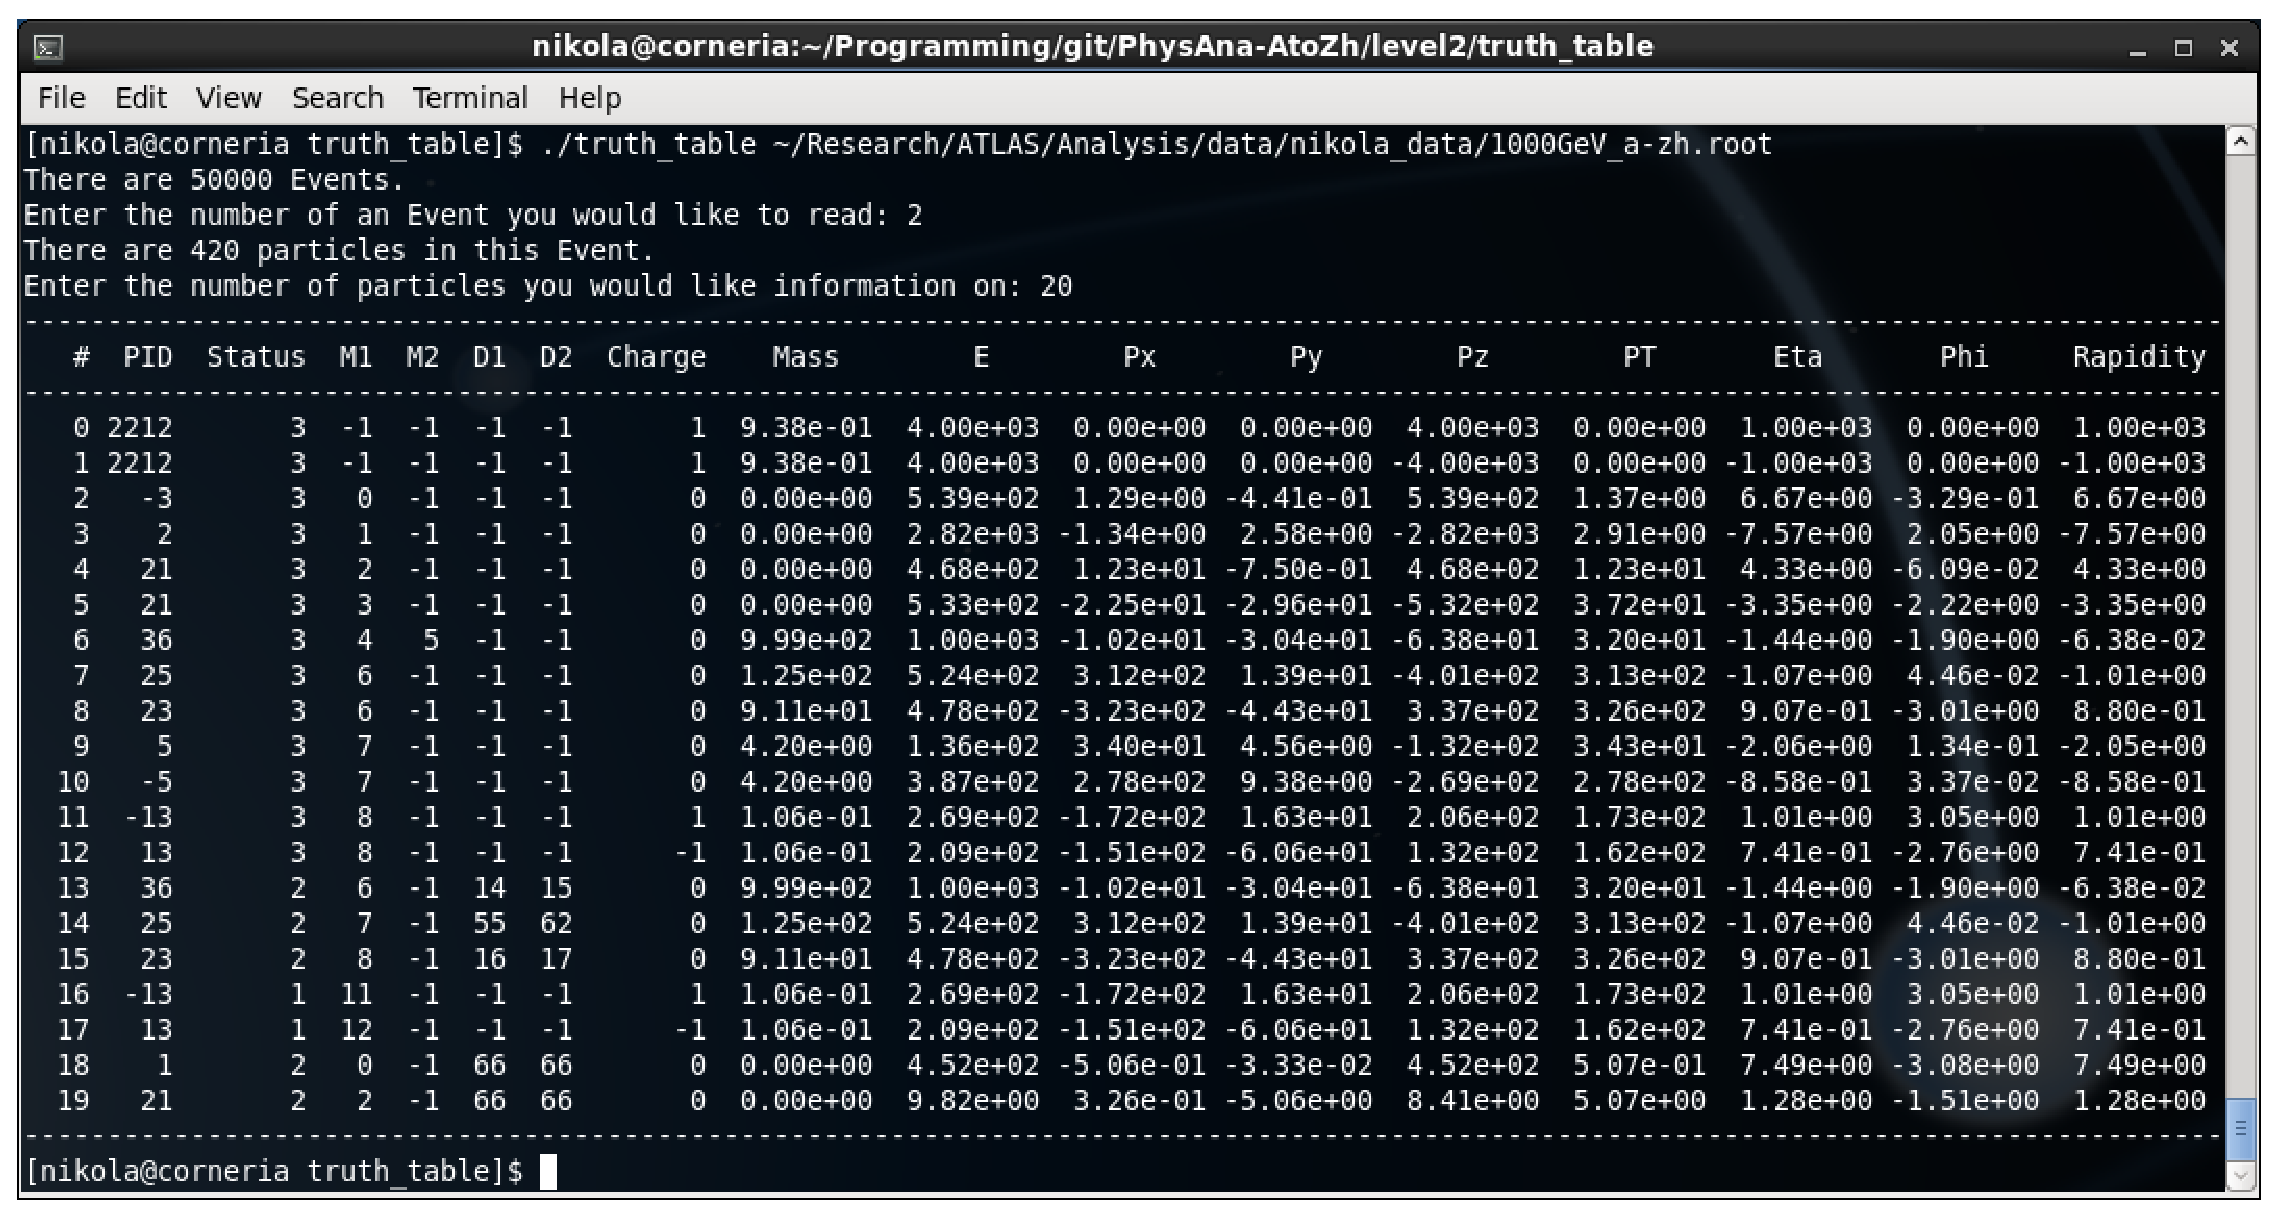
\includegraphics[width = \linewidth]{truth_table_output.eps}
		\end{figure}
	\end{frame}
%%%%%%%%%%%%%%%%%%%%%%%%%%%%%%%%%%%%%%%%%%%%%%%%%%%%%%%%%%%%%%%%%%%%%%%%%%%%%%%%%%%%%%%%%%%%%%%%%%%%%%%%%%%%%%%%%%%%%%%%%%%%%%%%%%%%%%%%%%%%%%%%%%%%%%%%%%%%%%%%%%%%%%%%%%%%%%%%%%%%%%%%%%%%%%%%%%%
	\begin{frame}{Truth Particle Details, PID, M1, M2, D1, D2}
Let's discuss some of the output information.

\bigskip

		\begin{itemize}
\item<1->PID: This stands for "Particle ID," and refers to what type of particle you are looking at. For example "13" refers to muons and "23" refers to Z bosons. More PID definitions can be found at the following website.

\bigskip

\url{http://www.physics.ox.ac.uk/CDF/Mphys/old/notes/pythia_codeListing.html}

\bigskip

\item<1->M1, M2, D1, D2: These refer to the index of the mother and daughter particles. For example, the mother of the 12th particle in the output table (a muon) is the 8th particle in the table (a Z boson).
		\end{itemize}

\bigskip
	\end{frame}
%%%%%%%%%%%%%%%%%%%%%%%%%%%%%%%%%%%%%%%%%%%%%%%%%%%%%%%%%%%%%%%%%%%%%%%%%%%%%%%%%%%%%%%%%%%%%%%%%%%%%%%%%%%%%%%%%%%%%%%%%%%%%%%%%%%%%%%%%%%%%%%%%%%%%%%%%%%%%%%%%%%%%%%%%%%%%%%%%%%%%%%%%%%%%%%%%%%
	\begin{frame}{Truth Particle Details, Status}

		\begin{itemize}
\item<1->Status 1: This refers to particles after the MadGraph simulation, but before Pythia simulates parton showers.
\item<1->Status 2: This refers to intermediate particles between Status 1 and Status 3.
\item<1->Status 3: This refers to final state particles, after Pythia simulates parton showers.
		\end{itemize}

\bigskip
	\end{frame}
%%%%%%%%%%%%%%%%%%%%%%%%%%%%%%%%%%%%%%%%%%%%%%%%%%%%%%%%%%%%%%%%%%%%%%%%%%%%%%%%%%%%%%%%%%%%%%%%%%%%%%%%%%%%%%%%%%%%%%%%%%%%%%%%%%%%%%%%%%%%%%%%%%%%%%%%%%%%%%%%%%%%%%%%%%%%%%%%%%%%%%%%%%%%%%%%%%%
	\begin{frame}{truth\_histogram}
		\begin{itemize}
\item<1->With this basic understanding of truth particles and Event structure, let's now discuss some truth particle analysis.

\bigskip

\item<1->truth\_histogram is a program which creates a histogram to display the distribution of a truth particle variable. For example, it can be quickly modified to output histograms of truth electron PT. The code for truth\_histogram can be located in the tutorial git repository at the following url.

\bigskip

\url{https://github.com/schsu/PhysAna-AtoZh/tree/master/level2/truth_histogram}

\bigskip

\item<1->I will present and explain some plots output from truth\_histogram in the following slides, and describe how they motivate Event cuts and further analysis.
		\end{itemize}
	\end{frame}
%%%%%%%%%%%%%%%%%%%%%%%%%%%%%%%%%%%%%%%%%%%%%%%%%%%%%%%%%%%%%%%%%%%%%%%%%%%%%%%%%%%%%%%%%%%%%%%%%%%%%%%%%%%%%%%%%%%%%%%%%%%%%%%%%%%%%%%%%%%%%%%%%%%%%%%%%%%%%%%%%%%%%%%%%%%%%%%%%%%%%%%%%%%%%%%%%%%
	\begin{frame}{Status 3 Lepton Multiplicity}
		\begin{columns}
			\begin{column}{0.5\textwidth}
				\includegraphics[width = \linewidth]{truth_electron_3_multiplicity.eps}
			\end{column}
			\begin{column}{0.5\textwidth}
				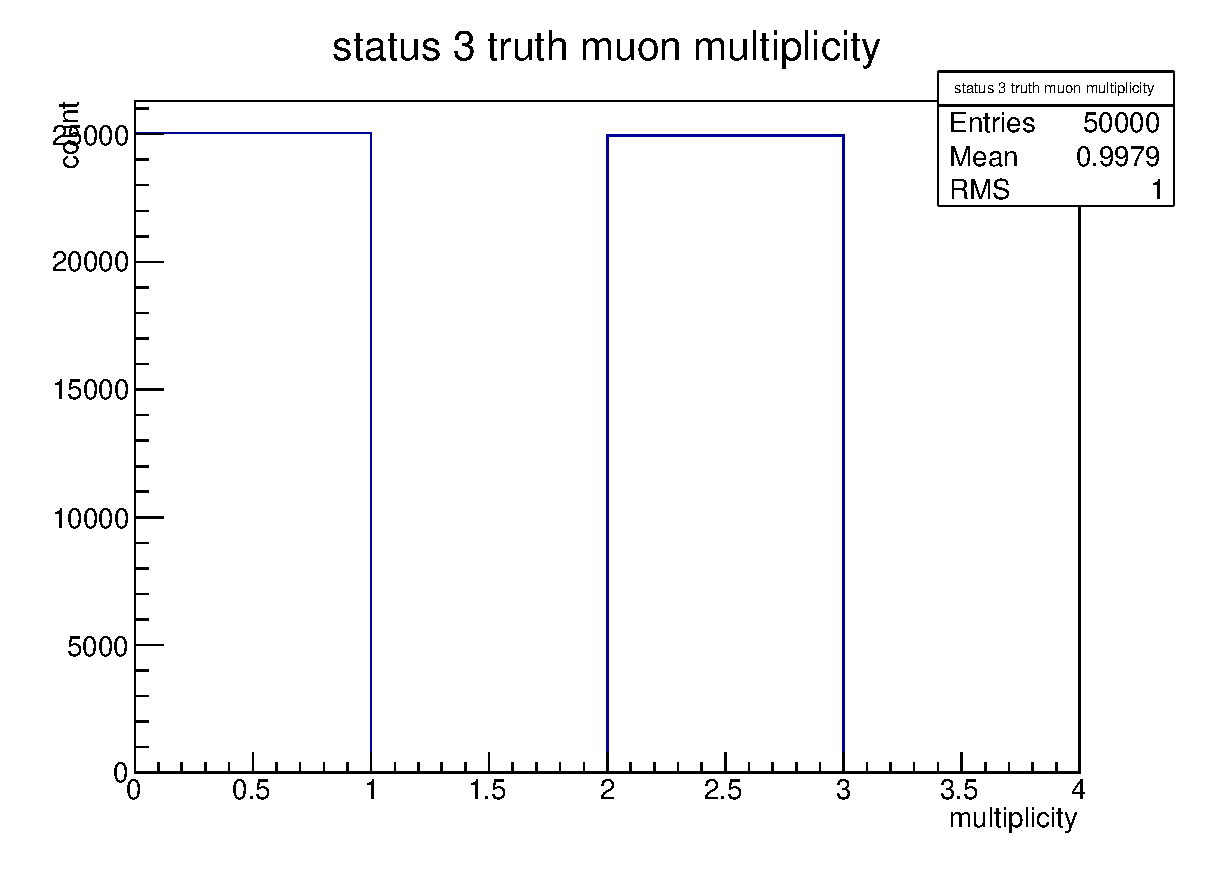
\includegraphics[width = \linewidth]{truth_muon_3_multiplicity.eps}
			\end{column}
		\end{columns}
Here we see the multiplicity of status 3 electrons and muons. This verifies that there are indeed either 0 or 2 leptons per event.
	\end{frame}
%%%%%%%%%%%%%%%%%%%%%%%%%%%%%%%%%%%%%%%%%%%%%%%%%%%%%%%%%%%%%%%%%%%%%%%%%%%%%%%%%%%%%%%%%%%%%%%%%%%%%%%%%%%%%%%%%%%%%%%%%%%%%%%%%%%%%%%%%%%%%%%%%%%%%%%%%%%%%%%%%%%%%%%%%%%%%%%%%%%%%%%%%%%%%%%%%%%
	\begin{frame}{Status 3 and Status 1 Electron PT}
		\begin{columns}
			\begin{column}{0.5\textwidth}
				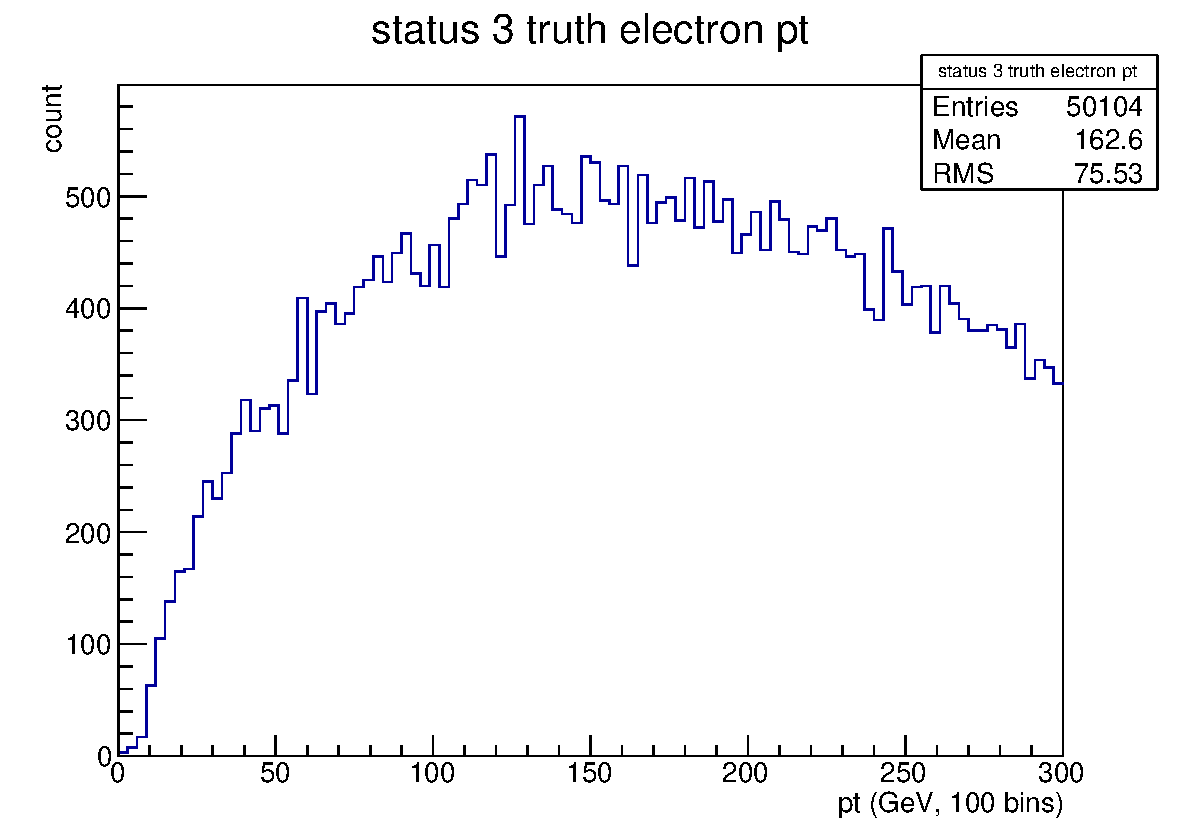
\includegraphics[width = \linewidth]{truth_electron_3_pt.eps}
			\end{column}
			\begin{column}{0.5\textwidth}
				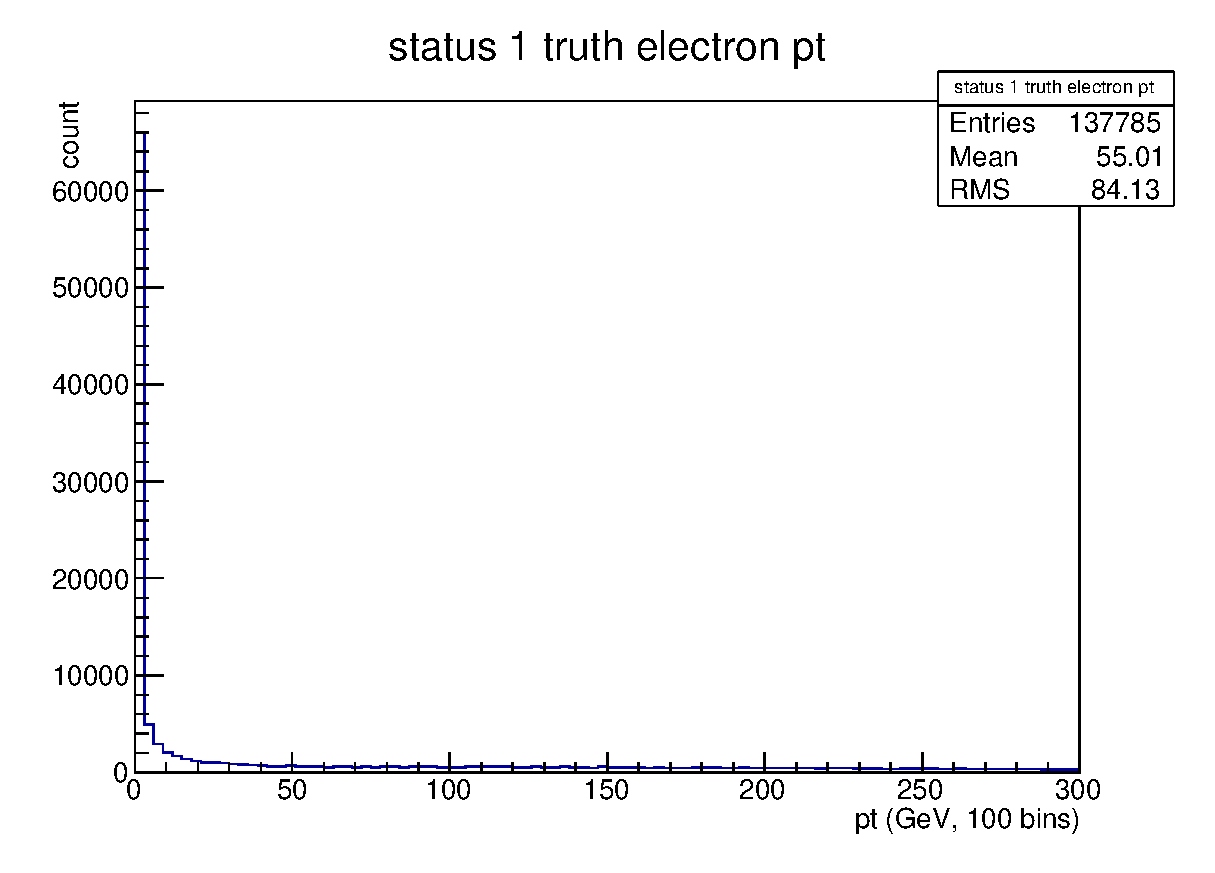
\includegraphics[width = \linewidth]{truth_electron_1_pt.eps}
			\end{column}
		\end{columns}
From these plots, we can infer that many electrons were produced when Pythia simulated parton showers, and that these new electrons have a low PT distribution. This is early motivation for a PT cut.

\bigskip

To verify that these electrons come from parton showers, you can use truth\_table to carefully peruse decay chains, or you can use ROOT to carefully loop through the decay chain, using the M1 and M2 variables.
	\end{frame}
%%%%%%%%%%%%%%%%%%%%%%%%%%%%%%%%%%%%%%%%%%%%%%%%%%%%%%%%%%%%%%%%%%%%%%%%%%%%%%%%%%%%%%%%%%%%%%%%%%%%%%%%%%%%%%%%%%%%%%%%%%%%%%%%%%%%%%%%%%%%%%%%%%%%%%%%%%%%%%%%%%%%%%%%%%%%%%%%%%%%%%%%%%%%%%%%%%%
	\begin{frame}{Conclusion}
		\begin{itemize}
\item<1->This presentation should be a good overview of the methods, goals, and results of Level 1 and Level 2 of the AZH Tutorial.

\bigskip

\item<1->The details of carrying out the simulations and analysis presented here are described in the main AZH Tutorial pdf document and the analysis source code found on the AZH Tutorial git repositories.

\bigskip

\item<1->If you are just starting out with analysis, or would like a refresher on the details, please refer to these resources.
		\end{itemize}
\bigskip

Thanks!
	\end{frame}
%%%%%%%%%%%%%%%%%%%%%%%%%%%%%%%%%%%%%%%%%%%%%%%%%%%%%%%%%%%%%%%%%%%%%%%%%%%%%%%%%%%%%%%%%%%%%%%%%%%%%%%%%%%%%%%%%%%%%%%%%%%%%%%%%%%%%%%%%%%%%%%%%%%%%%%%%%%%%%%%%%%%%%%%%%%%%%%%%%%%%%%%%%%%%%%%%%%
\end{document}
